\documentclass[12pt,a4paper]{article} 

\usepackage{titlesec}
\usepackage{color}
\usepackage[utf8]{inputenc}
\usepackage[english]{babel}
\usepackage[T1]{fontenc}
\usepackage{graphicx}
\graphicspath{{Images/}}
\usepackage{eso-pic} 
\usepackage{subfig} 
\usepackage{caption} 
\usepackage{transparent}
\usepackage{amsmath}
\usepackage{amsthm}
\usepackage{bm}
\usepackage[overload]{empheq}  
\usepackage{tabularx}
\usepackage{longtable}
\usepackage{colortbl}
\usepackage{algorithm}
\usepackage{algorithmic}
\usepackage[colorlinks=true,linkcolor=black,anchorcolor=black,citecolor=black,filecolor=black,menucolor=black,runcolor=black,urlcolor=black]{hyperref} 
\usepackage{cleveref}
\usepackage[square, numbers]{natbib} 
\bibliographystyle{unsrt}
\usepackage{appendix}
\usepackage{enumitem}
\usepackage{amsthm,thmtools,xcolor} 
\usepackage{comment} 
\usepackage{fancyhdr} 
\usepackage{lipsum} 
\usepackage{tcolorbox} 
\newcommand{\bea}{\begin{eqnarray}} 
\newcommand{\eea}{\end{eqnarray}}
\newcommand{\e}[1]{\times 10^{#1}}  
\newcommand{\mathbbm}[1]{\text{\usefont{U}{bbm}{m}{n}#1}} 
\newcommand{\pdev}[2]{\frac{\partial#1}{\partial#2}}

% Configuration package
\usepackage[bottom=2.0cm,top=2.0cm,left=2.0cm,right=2.0cm]{geometry}
\raggedbottom 

% Create color bluePoli (-> manuale grafica coordinata:  https://www.polimi.it/fileadmin/user_upload/il_Politecnico/grafica-coordinata/2015_05_11_46xy_manuale_grafica_coordinata.pdf)
\definecolor{bluePoli}{cmyk}{0.4,0.1,0,0.4}

% Custom theorem environments
\declaretheoremstyle[
  headfont=\color{bluePoli}\normalfont\bfseries,
  bodyfont=\color{black}\normalfont\itshape,
]{colored}

\captionsetup[figure]{labelfont={color=bluePoli}} % Set colour of the captions
\captionsetup[table]{labelfont={color=bluePoli}} % Set colour of the captions
\captionsetup[algorithm]{labelfont={color=bluePoli}} % Set colour of the captions

\theoremstyle{colored}
\newtheorem{theorem}{Theorem}[section]
\newtheorem{proposition}{Proposition}[section]

% Enhances the features of the standard "table" and "tabular" environments.
\newcommand\T{\rule{0pt}{2.6ex}}
\newcommand\B{\rule[-1.2ex]{0pt}{0pt}}

% Algorithm description
\newcounter{algsubstate}
\renewcommand{\thealgsubstate}{\alph{algsubstate}}
\newenvironment{algsubstates}{
    \setcounter{algsubstate}{0}%
    \renewcommand{\STATE}{%
    \stepcounter{algsubstate}%
    \Statex {\small\thealgsubstate:}\space}
    }{}
    
% Custom theorem environment
\newcolumntype{L}[1]{>{\raggedright\let\newline\\\arraybackslash\hspace{0pt}}m{#1}}
\newcolumntype{C}[1]{>{\centering\let\newline\\\arraybackslash\hspace{0pt}}m{#1}}
\newcolumntype{R}[1]{>{\raggedleft\let\newline\\\arraybackslash\hspace{0pt}}m{#1}}

% Custom itemize environment
\setlist[itemize,1]{label=$\bullet$}
\setlist[itemize,2]{label=$\circ$}
\setlist[itemize,3]{label=$-$}
\setlist{nosep}

% Create command for background pic
\newcommand\BackgroundPic{% Adding background picture
	\put(237,365){
	    \parbox[b][\paperheight]{\paperwidth}{%
	    \vfill
		\centering
		\transparent{0.4}
		
\includegraphics[width=0.44\paperwidth]{raggiera_polimi.eps}%
		\vfill}
		}
}

% Set indentation
\setlength\parindent{0pt}

% Custom title commands
\titleformat{\section}
{\color{bluePoli}\normalfont\Large\bfseries}
{\color{bluePoli}\thesection.}{1em}{}
\titlespacing*{\section}
{0pt}{3.3ex}{3.3ex}

\titleformat{\subsection}
{\color{bluePoli}\normalfont\large\bfseries}
{\color{bluePoli}\thesubsection.}{1em}{}
\titlespacing*{\subsection}
{0pt}{3.3ex}{3.3ex}

% Custom headers and footers
\pagestyle{fancy}
\fancyhf{}
      
\fancyfoot{}
\fancyfoot[C]{\thepage} % page
\renewcommand{\headrulewidth}{0mm} % headrule width
\renewcommand{\footrulewidth}{0mm} % footrule width

\makeatletter
\patchcmd{\headrule}{\hrule}{\color{black}\hrule}{}{} % headrule
\patchcmd{\footrule}{\hrule}{\color{black}\hrule}{}{} % footrule
\makeatother

% -> title of your work
\renewcommand{\title}{KANs: Kolmogorov-Arnold Networks}
% -> author name and surname
\renewcommand{\author}{Pasqual Matteo Romilio}
% -> MSc course
\newcommand{\course}{Master's degree in Computer Science Engineering }
% -> advisor name and surname
\newcommand{\advisor}{Prof. Edie Miglio}
% -> author ID
\newcommand{\ID}{10765765}
% -> academic year
\newcommand{\YEAR}{2024-2025}
% -> abstract (only in English)
\renewcommand{\abstract}{ 
Inspired by the Kolmogorov-Arnold representation theorem, we propose Kolmogorov-Arnold Networks (KANs) as promising alternatives to Multi-Layer Perceptrons (MLPs). Unlike MLPs, which utilize fixed activation functions on nodes (\textit{"neurons"}), KANs employ learnable spline-based activation functions on edges (\textit{"weights"}), eliminating the need for linear weights. This design enables KANs to overcome MLPs in accuracy and interpretability. Empirically, smaller KANs achieve comparable or better accuracy than larger MLPs in function fitting, supported by faster neural scaling laws. Moreover, KANs excel in interpretability, allowing intuitive visualization and interaction, making them valuable collaborators for rediscovering mathematical and physical laws. By demonstrating superior performance in accuracy and usability, KANs offer a novel framework for enhancing modern deep-learning models that depend heavily on MLPs.
}

% -> key-words (only in English)
\newcommand{\keywords}{}

%------------------
%	BEGIN OF YOUR DOCUMENT
%------------------
\begin{document}
% DO NOT REMOVE SPACES BETWEEN LINES!

\AddToShipoutPicture*{\BackgroundPic}

\hspace{-0.6cm}
\includegraphics[width=0.6\textwidth]{logo_polimi_ing_indinf.eps}

\vspace{-1mm}
\Large{\textbf{\color{bluePoli}{\title}}}\\

\vspace{-0.2cm}
\fontsize{0.3cm}{0.5cm}\selectfont \bfseries \textsc{\color{bluePoli}  Project of Numerical Analysis for Machine Learning \\ \course}\\

\vspace{-0.2cm}
\large{\textbf{\author, \ID}}

\small \normalfont

\vspace{11pt}

\centerline{\rule{1.0\textwidth}{0.4pt}}

\begin{center}
\begin{minipage}[t]{.26\textwidth}
\begin{minipage}{.90\textwidth}
\noindent
\scriptsize{\textbf{Advisor:}} \\
\advisor \\
\\ % leave it if any co-advisor otherwise comment
\textbf{Academic year:} \\
\YEAR \\
\\
\end{minipage}
\end{minipage}% This must go next to `\end{minipage}`
\begin{minipage}{.74\textwidth}
\noindent \textbf{\color{bluePoli} Abstract:} {\abstract}
\end{minipage}
\end{center}

\vspace{15pt}

\begin{tcolorbox}[arc=0pt, boxrule=0pt, colback=bluePoli!60, width=\textwidth, colupper=white]
    \textbf{} \keywords
\end{tcolorbox}

\vspace{12pt}

%--------------
% PAPER
%--------------
\section{Introduction}
\label{sec:in}
Multi-layer perceptrons (MLPs), also known as fully-connected feedforward neural networks, are foundational building blocks of today’s deep learning models. The importance of MLPs can never be overstated, since they are the default models in machine learning for approximating non-linear functions, due to their expressive power guaranteed by the universal approximation theorem. 

However, are MLPs the best non-linear regressors we can build? Despite the prevalent use of MLPs, they have significant drawbacks. In transformers, for example, MLPs consume almost all non-embedding parameters and are typically less interpretable (relative to attention layers) without post-analysis tools.

We propose a promising alternative to MLPs, called Kolmogorov-Arnold Networks (KANs). 

Whereas MLPs are inspired by the universal approximation theorem, KANs are inspired by the Kolmogorov-Arnold representation theorem. Like MLPs, KANs have fully-connected structures. However, while MLPs place fixed activation functions on nodes “neurons”), KANs place learnable activation functions on edges (“weights”), as illustrated in Figure~\ref{fig:MLPKAN}. As a result, KANs have no linear weight matrices at all: instead, each weight parameter is replaced by a learnable 1D function parametrized as a spline. KANs’ nodes simply sum incoming signals without applying any non-linearities. 

One might worry that KANs are hopelessly expensive since each MLP’s weight parameter becomes KAN’s spline function. Fortunately, KANs usually allow much smaller computation graphs than MLPs embedding a 2-hidden-layer neural network.

Throughout this paper, we will show that KANs can lead to higher accuracy and improved interpretability over MLPs. We will show how, by leveraging the Kolmogorov-Arnold representation theorem, learnable activation functions and the absence of fixed-weight matrices allow KANs to efficiently capture complex relationships within the data\cite{KAN}.

\begin{figure}[H]
    \centering
    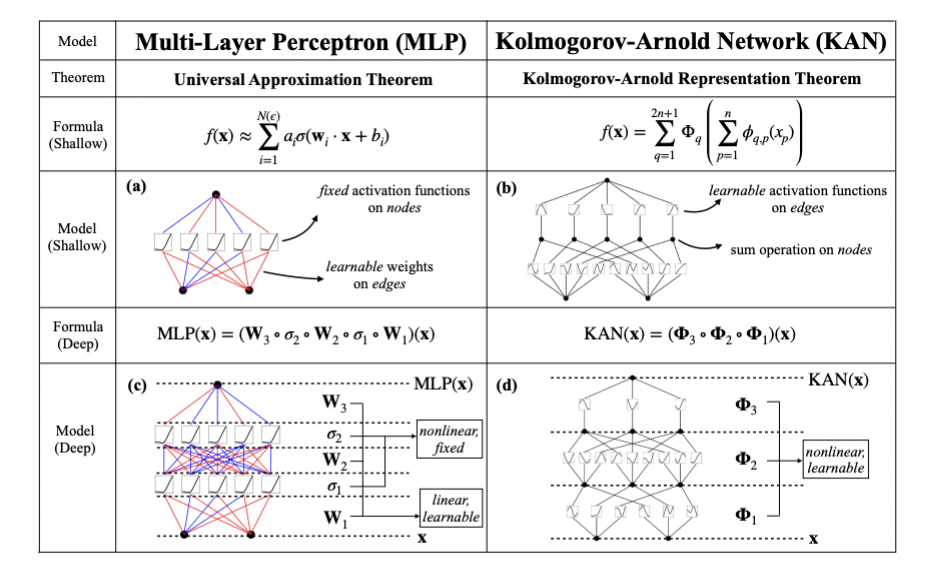
\includegraphics[width=0.8\linewidth]{Images/MLP-KAN.png}
    \caption{Multi-layer perceptrons (MLPs) vs Kolmogorov-Arnold Networks (KANs)}
    \label{fig:MLPKAN}
\end{figure}
\section{Kolmogorov-Arnold representation theorem}
\label{sec:ka}
Whereas Multi-layer perceptrons (MLPs) are inspired by the universal approximation theorem, Kolmogorov-Arnold Networks (KANs) are inspired by the Kolmogorov-Arnold representation theorem \cite{KAN}.

Firstly, we start with the basic concept that a neural network can be described as a multivariate continuous function $f: \Re^n \rightarrow \Re^m $ that maps an input vector $\textbf{x}\in \Re^n$ to an output vector $\textbf{y}\in \Re^m$ via a series of computations. In particular, both MLPs and KANs can be described as a multivariate continuous function $f: \Re^n \rightarrow \Re $ that maps an input vector $\textbf{x}\in \Re^n$ to an output value $y\in \Re$ via a series of computations: $f(x) \equiv KAN(x)$ \cite{book1NAML, book2NAML}.

As in MLP when input variables are combined linearly we have to standardize inputs passing from a domain $D \subset \Re^n$ to a compact domain $D \subset [0,1]^n $. A possibility is to apply an affine transformation to the data so that each feature will be normalized in $[0,1] \in 
 \Re$.

\subsection{Theorem}
We can now formally present and demonstrate the Kolmogorov-Arnold representation theorem. 

The Kolmogorov-Arnold representation theorem is essential for proving that any neural network that has one output (for instance MLPs) can always be rebuilt as two-hidden-layer KANs. In particular, the Kolmogorov-Arnold representation theorem states that if $f$ is a multivariate continuous function on a bounded domain, then it can be written as a finite composition of continuous functions of a single variable and the binary operation of addition \cite{KAtheorem, KArevisited}.

\begin{theorem}[Kolmogorov-Arnold representation theorem \cite{KAtheorem}] 
\label{Kolmogorov-Arnold}
Let $f$ be an arbitrary multivariate continuous function on a bounded domain $f:[0,1]^n -> \Re$, then $f$:

$$f(\textbf{x}) = f(x_1,x_2,...,x_n) = \sum_{q=1}^{2n+1} \Phi_q(\sum_{p=1}^n \phi_{q,p}(x_p))$$

with continuous one–dimensional inner functions $\phi_{q,p}:[0,1] -> \Re$ and continuous one–dimensional outer functions $\Phi_q:\Re -> \Re$.
\end{theorem} 

In a sense, they showed that the only true multivariate function is addition since every other function can be written using univariate functions and sum. The great advantage is that we have to learn only a polynomial number of 1D functions. However, these 1D functions can be non-smooth and even fractal, so they may not be learnable; in practice with spline function, we can approximate their shapes and achieve the accuracy that we want \cite{KAN}.

\subsection{KAN matrix form}
\label{sec:ma}
For a more formal definition, we define the representation matrix of the Kolmogorov-Arnold representation theorem ( $f: [0,1]^n \rightarrow \Re$ ) \cite{KAN}:

$$f(\textbf{x}) = \boldsymbol{\Phi_{out}} \times \boldsymbol{\Phi_{in} }\times \textbf{x}$$

where $\textbf{x} \in \Re^n$, $\boldsymbol{\Phi_{in}} \in \Re^{2n+1,n}$, and $\boldsymbol{\Phi_{out}} \in \Re^{2n+1}$:

\[
\boldsymbol{\Phi_{in}} = 
\begin{pmatrix}
\phi_{1,1}(\cdot) & \dots & \phi_{1,n}(\cdot) \\
\vdots &   & \vdots \\
\phi_{2n+1,1}(\cdot) & \dots & \phi_{2n+1,n}(\cdot)
\end{pmatrix},
\quad \boldsymbol{\Phi_{in}} = (\Phi_{1}(\cdot) \dots \Phi_{2n+1}(\cdot))
\]

\begin{figure}[H]
    \centering
    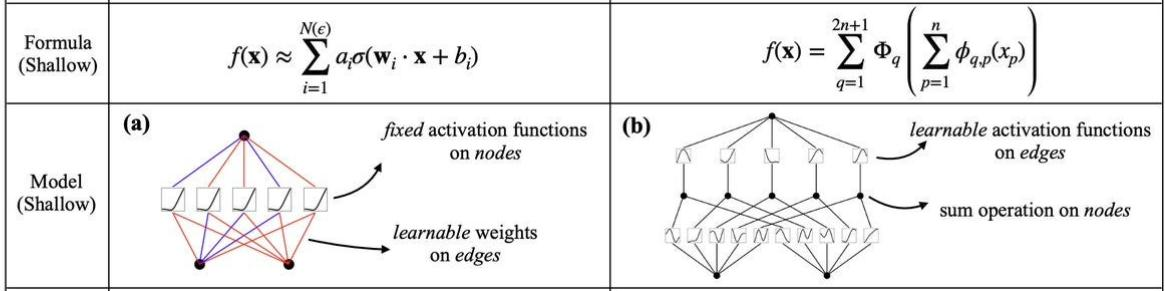
\includegraphics[width=0.8\linewidth]{Images/A.JPG}
    \caption{ MLPs vs KANs: Shallow model}
\end{figure}

\subsubsection{KAN layer form}
We notice that both matrices $\boldsymbol{\Phi_{in}}$ and $\boldsymbol{\Phi_{out}}$ are special cases of the matrix $\boldsymbol{\Phi} \in \Re^{n_{out},n_{in}}$ that represent a general Kolmogorov-Arnold layer. 

\[
\boldsymbol{\Phi} = 
\begin{pmatrix}
\phi_{1,1}(\cdot) & \dots & \phi_{1,n_{in}}(\cdot) \\
\vdots &   & \vdots \\
\phi_{n_{out},1}(\cdot) & \dots & \phi_{n_{out},n_{in}}(\cdot)
\end{pmatrix} 
\]

so each layer map his input $l$ $\textbf{x}_l$ to the output $\textbf{x}_{l+1}$ thought $\boldsymbol{\Phi}$:

\[
\textbf{x}_{l+1} = \boldsymbol{\Phi} \times \textbf{x}_l \Rightarrow
\textbf{x}_{l+1} = 
\begin{pmatrix}
\phi_{1,1}(\cdot) & \dots & \phi_{1,n_{in}}(\cdot) \\
\vdots &   & \vdots \\
\phi_{n_{out},1}(\cdot) & \dots & \phi_{n_{out},n_{in}}(\cdot)
\end{pmatrix} \textbf{x}_l
\]


Each layer has $n_{in}$ inputs and $n_{out}$ outputs and is mapped thought its respective layer matrix. In our case, the two layers are defined as follows:
\begin{itemize}
    \item Layer 1: $\boldsymbol{\Phi_{in}}$ has $\boldsymbol{\Phi}$ with $n_{in} = n$ and $n_{out} = 2n+1$
    \item Layer 2: $\boldsymbol{\Phi_{out}}$ has $\boldsymbol{\Phi}$ with $n_{in} = 2n+1$ and $n_{out} = 1$
\end{itemize}
\section{KAN}
Kolmogorov-Arnold networks are more expressive than their basic formulation from the Kolmogorov-Arnold representation theorem. 
According to the theorem, the layer requirements are two layers, with a corresponding depth of \(2n+1\) and \(n\). However, in practice, we can design networks with different topologies by adding layers or changing the definition of each layer \cite{KAN}. The key idea is to stack layers from the input to the output.

\subsection{Structure}
With these premises, we can construct various topologies of Kolmogorov-Arnold networks by simply stacking layers and following these rules:
\begin{itemize}
    \item A KAN, as all MPLs, is a directed acyclic graph (DAG). 
    \item Each KAN layer is fully connected to the preceding and succeeding layers apart from the first layer will only have a succeeding layer and the last layer will only have a preceding layer.
    \item Each KAN layer is not connected with other layers
    \item Each KAN layers connection $\textbf{x}_{l+1} = \boldsymbol{\Phi}_L \times \textbf{x}_l$ is defined by $\boldsymbol{\Phi_{L}} \in \Re^{n_{out},n_{in}}$ where $n_{in}$ is the dimension of the $\textbf{x}_l$ layer and $n_{out}$ is the dimension of the $\textbf{x}_l$ layer (Section~\ref{sec:ma}).
    \item Every edge of al layer $\phi_{l,q,p}$ is associated with a one-dimensional activation function. 
\end{itemize}

Let’s say we have a KAN with $L$ layers, where the $l^{th}$ layer has shape $n_{l+1}$, $n_l$ and has formula $\textbf{x}_{l+1} = \boldsymbol{\Phi} \times \textbf{x}_l $. Then the whole network will be represented by:

$$KAN(\textbf{x}) = \boldsymbol{\Phi_{L-1}} \times \dots \times \boldsymbol{\Phi_{1}} \times \boldsymbol{\Phi_{0}} \times \textbf{x}$$

We can also rewrite the above equation as a series of summations, assuming the output dimension $n_L = 1$ and the associated multivariate
continuous function $f$:  $f(x) \equiv KAN(x)$:

$$f(\textbf{x}) = \sum_{i_{L-1}=1}^{n_{L-1}}  \phi_{L-1,i_L,i_{L-1}} (...(\sum_{i_1=1}^{n_{1}}  \phi_{1,i_2,i_{1}}(\sum_{i_0=1}^{n_{0}}  \phi_{0,i_1,i_{0}}(x_{i_0}))...)$$

The network structure will be only a series of matrix-matrix multiplication of $ \boldsymbol{\Phi_{L-1}}, \dots, \boldsymbol{\Phi_{1}},\boldsymbol{\Phi_{0}}$  while a MLPs was a series of linear transformations $W_l$ and non-linear transformations $\sigma$:

$$MLP(\textbf{x}) = \boldsymbol{W_{L-1}} \times \sigma \times \dots \times \boldsymbol{W_{1}} \times \sigma \times\boldsymbol{W_{0}} \times \textbf{x}$$

\begin{figure}[H]
    \centering
    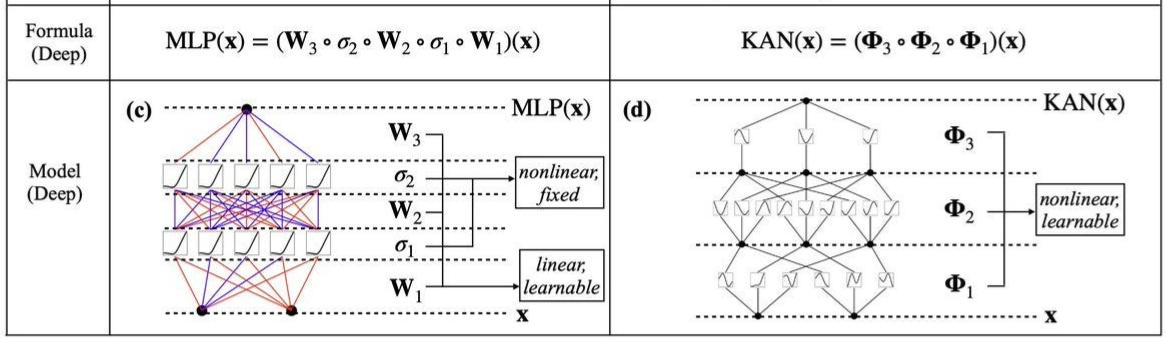
\includegraphics[width=0.8\linewidth]{Images/B.JPG}
    \caption{ MLPs vs KANs: Deep model }
\end{figure}

Finally, a KAN can be conceptualized as a structured stack of KAN layers. Each KAN layer can be represented as a fully connected layer where every edge is associated with a one-dimensional (1D) function. The critical components that need to be defined are the representation and training of these activation functions which are the only learnable part of the function.

\subsection{Activation functions}
While the equation to compute, given an input, the KAN's output appears very simple, ensuring that the activation functions are well-trained is more complex. The most efficient technique involves leveraging spline functions. These functions are particularly effective for approximating the complexity and the non-linearities of the 1D functions associated with the KAN layers. This approach enhances both the flexibility and trainability of the network \cite{KAN}.

Formally speaking, in KANs, every activation function $\phi_{l,q,p}(\cdot)$ is defined as follows:
$$\phi(x) = w_bb(x) + w_sspline(x) $$

where:
\begin{itemize}
    \item $w_b$ and $w_s$ are learnable weights; in principle are redundant since they can be absorbed into $b(x)$ and $spline(x)$, we still include these factors to better control the overall magnitude. In particular, $w_s$ is very useful to scale the spline function.
    \item $b(x)$ is a fixed function called residual connection function defined by the silu function $b(x) = silu(x) = \frac{x}{1+e^{-x}}$. It is the counterpart of biases in MLPs.
    \item $spline(x)$ that is the learnable function where the real power of KANs came from. In most of the cases is parametrized as a linear combination of B-splines functions ($B_i$) and defining $c_i$s the learnable B-splines points and $k$ is the spline order $spline(x)= \sum_i^k c_iB_i(x)$.
\end{itemize}

\subsection{Bézier and B-splines functions}
Given the spline function now we have to define its shape. In literature, two main classes of functions are designed for KANs:
\begin{itemize}
    \item Bézier functions which consider all the domains but are complex to train \cite{bezier}
    \item B-splines functions which consider only a local domain but are easy to train \cite{kan_intro}.
\end{itemize}

The problem we are going to solve is that the spline function should pass through some tag points that will be adjusted during the training phase. To solve it let's consider a dual problem: imagine a character $C$ must pass through $n$ points $(P_1, \dots,P_n)$. The most obvious way to traverse them is to go straight from $P_i$ to $P_{i+1}$ but this movement does not appear natural because we desire a smooth traversal movement that can be described as $(n-1)$-degree polynomial as in Figure~\ref{fig:bezier}.  
\begin{figure}[H]
    \centering
    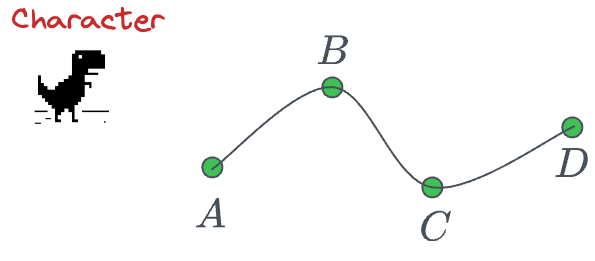
\includegraphics[width=0.5\linewidth]{Images/bezier.png}
    \caption{Example of 4-degree polynomial curve}
    \label{fig:bezier}
\end{figure}

The naive way to implement it is to define a function $h(x): \Re \to \Re$:

$$h(x) = a_{n-1}x^{n-1} + a_{n-2}x^{n-2} + \dots + a_1x +a_0 $$

then we can substitute points $(P_1, \dots,P_n)$ into the function $h$ and determine the values of the coefficients $(a_0, \dots,a_{n-1})$. Now we realize that we have to solve $N$ equations to determine the coefficients. Solving such a system of linear equations will be computationally expensive and almost infeasible for KANs. For this reason, we choose Bézier or B-splines functions.

\subsubsection{Bézier}
Bézier curves solve the problem more smartly. They provide a way to represent a smooth curve that passes near a set of control points without needing to solve a large system of equations as in Figure~\ref{fig:bezier2}.   
\begin{figure}[H]
    \centering
    \subfloat{%
        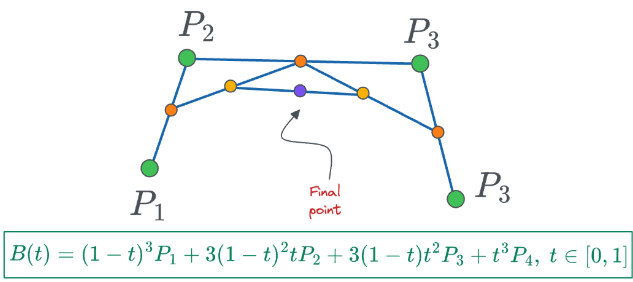
\includegraphics[width=0.55\linewidth]{Images/bezier2.png}%
        \label{fig:bezier2a}%
    }
    \hfill
    \subfloat{%
        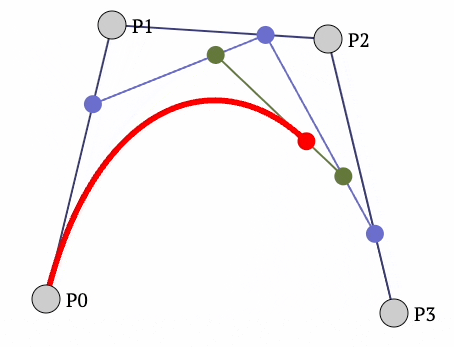
\includegraphics[width=0.30\linewidth]{Images/bezier3.png}%
        \label{fig:bezier2b}%
    }
    \caption{Example of 4-degree bezier curves}
    \label{fig:bezier2}
\end{figure}


We define the Bézier curve $b(t): \Re \to \Re$ noticing from low $n$ polynomials as in Figure~\ref{fig:bezier2} that the coefficients match with the binomial coefficients of $(1+t)^n$. Then we can derive the binomial definition of the Bézier curve as:

\[
\mathbf{b}(t) = \sum_{i=0}^n \binom{n}{i} (1-t)^{n-i} t^i \mathbf{P}_i, \quad t \in [0, 1]
\]

However, the problem is still the same as before. Having $N$ data points will result in a polynomial of degree $N-1$, which will be computationally expensive.

\subsubsection{B-splines}
B-splines provide a more efficient way to represent curves, especially when we deal with a large number of data. Unlike high-degree polynomials, B-splines use a series of lower-degree polynomial segments, which are connected smoothly.
In other words, instead of extending Bézier curves to tens of hundreds of data points, which leads to an equally high degree of the polynomial, we use multiple lower-degree polynomials and connect them to form a smooth curve as in Figure~\ref{fig:bezier4}.

\begin{figure}[H]
    \centering
    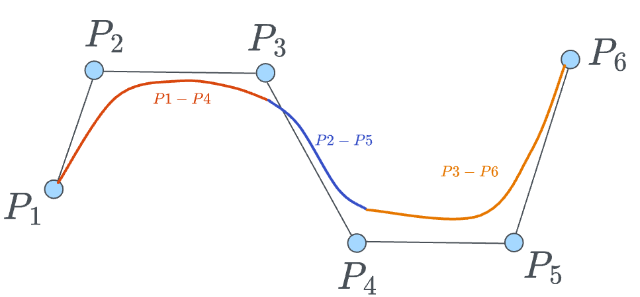
\includegraphics[width=0.5\linewidth]{Images/bezier4.png}
    \caption{Example of 6-degree B-spline curve}
    \label{fig:bezier4}
\end{figure}

When we have $n$ control points and we create $k$ degree polynomial Bézier curves, we get $(n-k)$ Bézier curves in the final Bsplines. We ensure also a certain continuity condition at the points where the curves meet:
\begin{itemize}
    \item Position Continuity: $C^0$ Continuity 
    \item Tangent Continuity: $C^1$ Continuity  
    \item Curvature Continuity: $C^2$ Continuity 
\end{itemize}

Similar to Bézier curves, we define the B-spline curve \( B(x): \Re \to \Re \) as a linear combination of the learnable position of points \( P_i \) and their associated non-learnable basis functions \( N_{i,k} \):


\[
\mathbf{B_i}(x) = \sum_{i=0}^n P_i N_{i,k} \Rightarrow \textbf{splines}(x ) = \sum_{i=0}^k c_i B_{i}(x) = \sum_{i=0}^k c_i \sum_{i=0}^n P_i N_{i,k}
\]

Finally, we have defined spline as a B-spline function linear combination. This is best choice for KANs, even though they consider only a local domain, because their strength lies in their easy trainability, even as the number of points increases.

\subsection{Initialization and training}
After defining all the components of the network and their connections, we will explain how training is performed. The key idea behind the training process is to make the positions of the control points $P_i$ in the activation function learnable, allowing the model to adapt and learn any arbitrary shape for the activation function that best fits the data. \cite{KAN,kan_intro}

\subsubsection{Inizialization}
The only trainable part of a KAN network is the set of activation functions. In particular, for each activation function, we will train the weights $w_b$ and $w_s$ and the spline function $spline(x)$. 
\begin{itemize}
    \item We initialize the scaling factor for the spline function at 1: $w_s=1$. 
    \item Each spline function is initialized with $spline(x) \approx 0$.  This is done by drawing B-spline coefficients $c_i \sim \mathcal{N}(0, \sigma^2)$ with a small $\sigma$ around 0.1. It's likely used to ensure symmetry and stability in early training stages.
    \item We initialize the scaling factor for the residual connection function with the Xavier initialization as in MLPs: $w_b \sim \mathcal{U}\left[-\sqrt{\frac{6}{n_{\text{in}} + n_{\text{out}}}}, \sqrt{\frac{6}{n_{\text{in}} + n_{\text{out}}}}\right]$ where $n_{in}$ and $n_{out}$ are specific for any layers.
\end{itemize}

\subsubsection{Training}
Once the initialization has been defined, the KAN can be trained just like any other neural network. In particular for $N_{epochs}$ we will perform:
\begin{itemize}
    \item Forward propagation computing $KAN(\textbf{x}) = \boldsymbol{\Phi_{L-1}} \times \dots \times \boldsymbol{\Phi_{1}} \times \boldsymbol{\Phi_{0}} \times \textbf{x}$
    \item Backword propagation computing the loss with the LSM or the cross-entropy method and then adjusting $w_b$ and $ splines(x)$ with some method as GD, SGD, NM, BFGS, or others. The parameter $w_s$, which is a scale factor, will only be modified if the spline activation values evolve out of the fixed region during training.
\end{itemize}

\subsection{Hyperparameters and complexity}
The hyperparameters of a Kolmogorov-Arnold network are:
\begin{itemize}
    \item \textbf{L}: the depth of the KAN
    \item \textbf{N} $ \in \{\textbf{n}_0$, ... ,$\textbf{n}_l\}$: width of each layer
    \item \textbf{k}: each spline is a linear combination of k B-splines. Usually, k is very small for instance $k=3$.
    \item \textbf{G}: each B-splines has G control points
\end{itemize}

Then a KAN with hyperparameters \textbf{L},\textbf{N},\textbf{G},\textbf{k}, considering $N$ as the biggest $n_i \in N$, we will have in total $O(N^2L(G + k))  \simeq O(N^2LG)$ parameters. In contrast, an MLP with hyperparameters \textbf{L, N} needs only  $O(N^2L)$ parameters, which appears to be more efficient than KAN. Fortunately, KANs usually require much smaller N than MLPs, which not only saves parameters but also achieves better generalization and facilitates interpretability \cite{KAN}. 

\subsubsection{Performance}
The most important Paper~\cite{KAN} has presented many performance-related results that compare the performance of KANs with MLP on various dummy/toy datasets. We will demonstrate that KANs are more effective when we want to perform non-linear regression or PDE solving.

In Figure~\ref{fig:re} the toy datasets are defined as follows:
\begin{enumerate}
    \item $f(x) = J_0(20x)$ (Bessel function): Represented by a $KAN(L=1,N=[1,1])$.
    \item $f(x, y) = e^{\sin(\pi x)+y^2}$: Represented by a $KAN(L=3,N=[2, 1, 1])$.
    \item $f(x, y) = xy$: Represented by a $KAN(L=3,N=[2, 2, 1])$.
    \item $f(x1_,\dots , x_{100}) = e^{\frac{1}{100} 
    \sum_{i=1}^{100} \sin^2(\frac{\pi x_i}{2})}$: Represented by a $KAN(L=3,N=[100, 1, 1])$.

    \item $f(x_1, x_2, x_3, x_4) = e^ {\sin(x_1^2 + x_2^2)+ \sin(x_3^2 + x_4^2)}$ : Represented by a $KAN(L=3,N=[4,4, 2, 1])$.
\end{enumerate}

We train these KANs by increasing grid points every 200 steps, in total covering

$G =\{3, 5, 10, 20, 50, 100, 200, 500, 1000\}$. We train MLPs with different depths and widths as baselines. Both MLPs and KANs are trained with LBFGS for 1800 steps in total.


\begin{figure}[H]
    \centering
    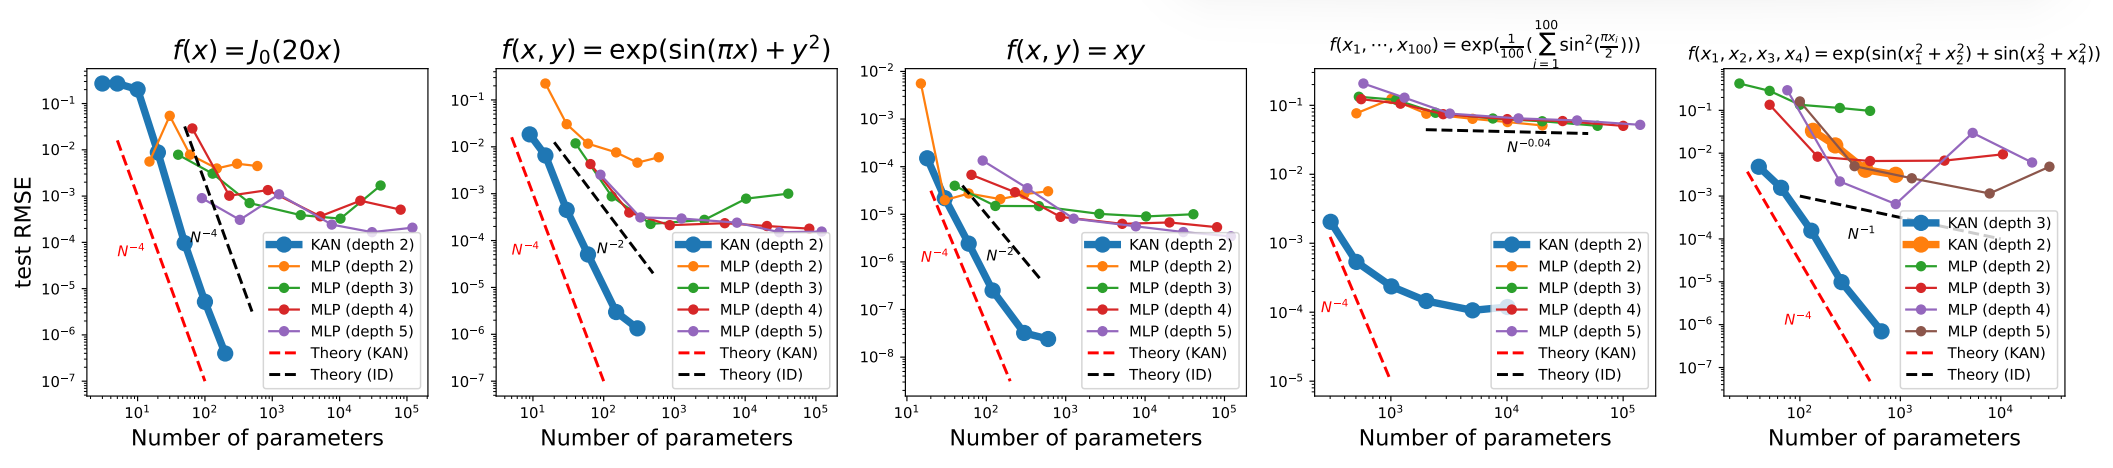
\includegraphics[width=0.95\linewidth]{Images/result.png}
    \caption{Results for KAN with toy dataset}
    \label{fig:re}
\end{figure}

In all the plots we can see that
\begin{itemize}
    \item KANs consistently outperform MLPs, achieving significantly lower test loss across a range of parameters, and at much lower network depth (number of layers).
    \item KANs demonstrate superior efficiency, with steeper declines in loss, particularly noticeable with fewer parameters.
    \item MLP's performance almost stagnates with increasing the number of parameters.
    \item The theoretical lines $N^{-4}$ for KAN and $N^{-2}$ for ideal models (ID), show that KANs closely follow their expected theoretical performance.
\end{itemize}
\subsection{Advanced Techniques}
Kolmogorov-Arnold networks can employ several advanced techniques to simplify the computation of the entire network reducing the time and space complexities. The main techniques are sparsification, pruning, and symbolification \cite{KAN}. 

Figure~\ref{fig:advanced} presents an example of advanced techniques (sparsification, prunig, and Symbolification).

\begin{figure}[H]
    \centering
    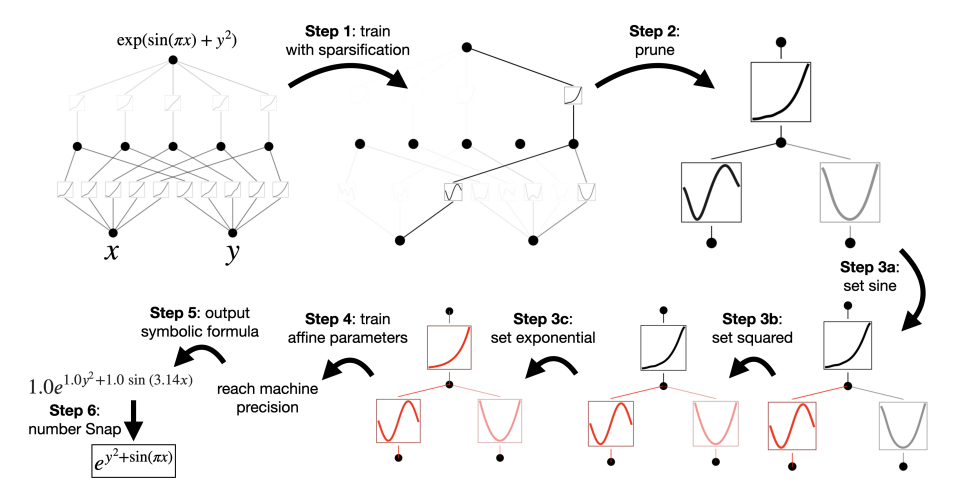
\includegraphics[width=0.85\linewidth]{LATEX//Images/advanced.png}
    \caption{Advanced KAN techniques}
    \label{fig:advanced}
\end{figure}

\subsubsection{Sparsification (Regularization)}
For MLPs, regularization, particularly L1 regularization of linear weights, is used to promote sparsity, thereby improving predictions. KANs can adopt this high-level concept, but two modifications are necessary:

\begin{enumerate}
    \item Since there are no linear weights in KANs, linear weights are replaced by learnable activation functions. Therefore, the L1 norm must be redefined for these activation functions.
    \item Experimentally, we find that L1 regularization alone is insufficient for sparsifying KANs. Instead, additional entropy regularization encourages the model to use activation functions with lower complexity and fewer degrees of freedom.
\end{enumerate}

We define the L1 norm of an activation function $\phi$ as its average magnitude over its $N_p$ inputs: $|\phi|_1$.

$$|\phi|_1 \equiv \frac{1}{N_p} \sum_{s=1}^{N_p} |\phi(x^{(s)})|$$

Then for a KAN layer $\boldsymbol{\Phi}$ with $n_{in}$ inputs and $n_{out}$ outputs, we define the L1 norm of $\boldsymbol{\Phi}$ to be the sum of L1 norms of all activation functions: $\boldsymbol{|\Phi|_1}$.

$$\boldsymbol{|\Phi|_1} \equiv \sum_{i=1}^{n_{in}}\sum_{j=1}^{n_{out}}|\phi_{i,j}|_1$$

In addition, as we have stated before, we define the regularization entropy of $\boldsymbol{\Phi}$ to be $S(\boldsymbol{\Phi})$.
$$S(\boldsymbol{\Phi}) \equiv -\sum_{i=1}^{n_{in}}\sum_{j=1}^{n_{out}} \frac{|\phi_{i,j}|_1}{\boldsymbol{|\Phi|_1}}\log(\frac{|\phi_{i,j}|_1}{\boldsymbol{|\Phi|_1}})$$

The total training objective $l_{total}$ is the prediction loss $l_{pred}$ plus L1 and entropy regularization of
all KAN layers where we define $\mu_1$, $\mu_2$ are relative magnitudes usually set to $\mu_1 = \mu_2 = 1$, and $\lambda$ controls overall regularization magnitude

$$l_{total} = l_{pred} + \lambda(\mu_1\sum_{l=0}^{L-1}\boldsymbol{|\Phi_l|_1} + \mu_2\sum_{l=0}^{L-1} S(\boldsymbol{\Phi_l}))$$

\subsubsection{Pruning}
After training with the sparsification penalty, we may also want to prune the network to a smaller subnetwork. We sparsify KANs at the node level (rather than at the edge level). For each node (say the $l^{th}$ neuron in the $l^{th}$ layer), we define its incoming and outgoing scores as $ I_{l, i}$ and $ O_{l, i}$.

$$ I_{l,i} = \max_k(|\phi_{l-1,i,k}|_1), \quad O_{l,i} = \max_j(|\phi_{l+1,j,i}|_1) $$

and consider a node to be important if both incoming and outgoing scores are greater than a threshold hyperparameter $\theta = 10^{-2}$ by default. Finally, all unimportant neurons are pruned reducing the network size.

\subsubsection{Symbolification}
In some cases, after pruning, we suspect that some activation functions are very similar to symbolic functions (such as $\cos(x)$, $\tanh(x)$, $e^x$, $\ln(x)$, etc.). The goal of Symbolification is to provide an interface to set the symbolic $\phi$ to its specified symbolic form. We will see how this leads to interpretability in Section~\ref{sec:interpre}.

Practically, we include a function $fix\_symbolic(l,i,j,f)$ that can set the activation at position $(l, i, j)$ to be $f$ if they are similar. 
However, we cannot simply set the activation function to the exact symbolic formula, since its inputs and outputs may have shifts and scaling. 
Therefore, we obtain the pre-activation values $x$ and post-activation values $y$ from samples and fit affine parameters $a$, $b$, $c$, and $d$ such that $y \approx c f(a x + b) + d$. The fitting is done by iterative search for $a$ and $b$, followed by linear regression to find $c$ and $d$. 

\subsection{Interpretability}
\label{sec:interpre}
One of the biggest drawbacks of multilayer perceptrons is their lack of interpretability. On the other hand, Kolmogorov-Arnold networks are more interpretable since they learn univariate functions at all levels, which can be inspected if needed. It is relatively easy to determine the structure learned by the network using those formulas \cite{kan_intro}.

Let's consider a KAN which is learning $f(x,y)=xy$ represented by $KAN(L=2,N=[4, 2])$.

\begin{figure}[H]
    \centering
    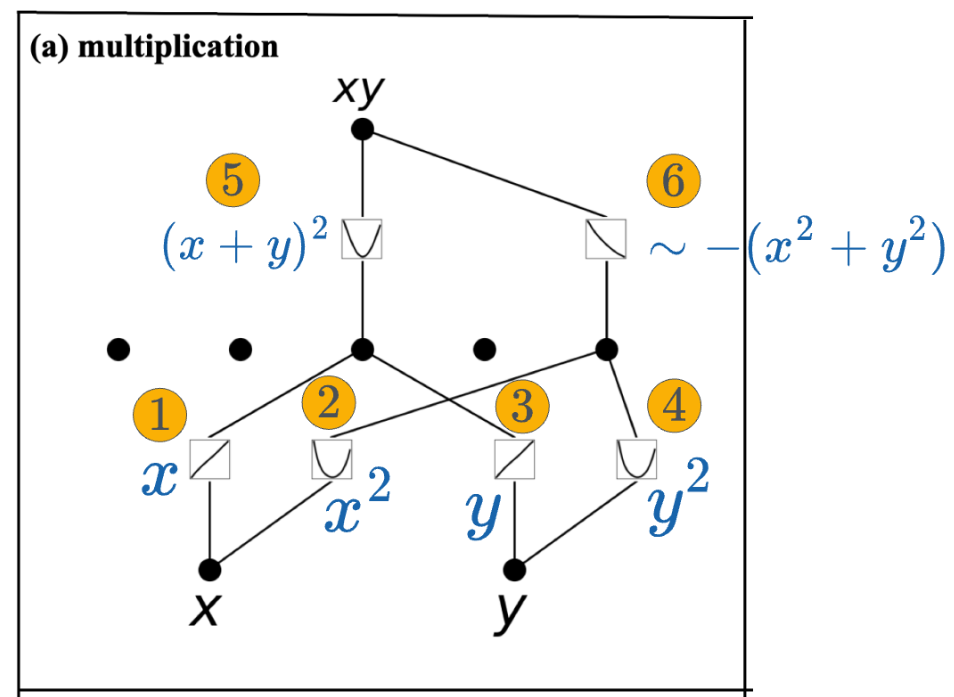
\includegraphics[width=0.5\linewidth]{LATEX//Images/interpr.png}
    \caption{Interpretation of $f(x,y)=xy$}
    \label{fig:interp}
\end{figure}

In Figure~\ref{fig:interp} inspecting the B-splines learned by KAN, we notice how the network is working.

In the first layer, both inputs $x$ and $y$ get transformed into their squares:
\begin{itemize}
    \item Activation \#1: map $x$ to $x$ $\Rightarrow \phi_{1,1}(k) = k $ 
    \item Activation \#2: map $x$ to $x^2$ $\Rightarrow \phi_{1,2}(k) = k^2$ 
    \item Activation \#3: map $y$ to $y$ $\Rightarrow \phi_{1,3}(k) = k$ 
    \item Activation \#4: map $y$ to $y^2$ $\Rightarrow \phi_{1,4}(k) = k^2$ 
\end{itemize}

In the second layer, we take the previous output and combine it as follows:
\begin{itemize}
    \item The sum of Activation \#1 and \#3, which is $(x+y)$, gets squared by activation \#5 and have $(x+y)^2$ as output then $\phi_{2,1}(k) = k^2$.

    \item The sum of Activation \#2 and \#4, which is $(x^2+y^2)$, gets negated by activation \#6 and have $-(x+y)$ as output then $\phi_{2,2}(k) = -k$.
\end{itemize}

Finally, the last sum will return us $2xy$.

$$(x+y)^2 - (x^2+y^2) = x^2+y^2 +2xy - x^2 -y^2 = 2xy   $$

The interpretation is almost finished apart from the scaling factor. In the real networks the parameters $w_s$ in the last layers are assigned to $0.5$ then the last sum will return us $xy$.

$$\frac{1}{2}(x+y)^2 - \frac{1}{2}(x^2+y^2) = \frac{1}{2}x^2+\frac{1}{2}y^2 +xy - \frac{1}{2}x^2 - \frac{1}{2}y^2 = xy   $$ 

We have proved that the network can be very easy to interpret by extracting the meaning from $\phi_{i,j}(k)$.

From the Paper \cite{KAN} in Figure~\ref{fig:interp2} we will see more examples of interpretability tasks.

\begin{figure}[H]
    \centering
    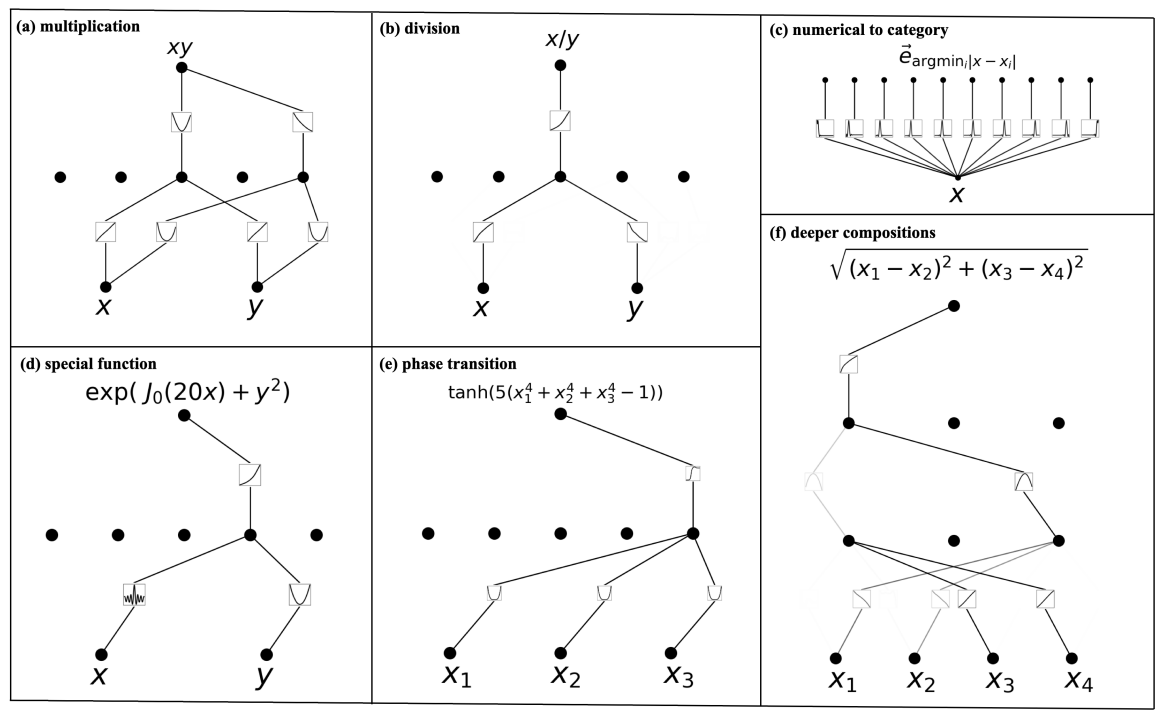
\includegraphics[width=0.8\linewidth]{LATEX//Images/interpr2.png}
    \caption{Interpretation of different functions}
    \label{fig:interp2}
\end{figure}
\section{Code}
\section{Conclusions}

Kolmogorov-Arnold Networks (KANs) offer an innovative approach to neural network architecture, diverging from Multi-layer Perceptrons (MLPs). Inspired by the Kolmogorov-Arnold representation theorem, KANs replace weight matrices and fixed activation functions with no weights and learnable spline-based functions that enhance expressiveness and adaptability. This unique design enables KANs to model complex, non-linear relationships with fewer parameters, leading to improved generalization and interpretability compared to MLPs. We have also demonstrated that KANs consistently outperform MLPs in non-linear regression and function approximation tasks, achieving lower test loss with reduced depth and complexity.

However, challenges persist in optimizing the training process for KANs. The reliance on spline activation functions introduces computational overhead, making KANs significantly slower than MLPs for comparable parameter counts. The current lack of mature optimization strategies for spline-based architectures further exacerbates this bottleneck. Despite these hurdles, advanced techniques such as sparsification, pruning, and symbolification have shown promise in reducing complexity, improving training efficiency, and providing a more interpretable network.

Looking forward, the potential for further improvement in KANs is immense. Research into accelerated training methods, more efficient spline representations, and scalable regularization techniques could unlock broader adoption and application of KANs across various machine learning tasks. Moreover, their ability to seamlessly integrate advanced techniques and provide symbolic interpretations of learned functions highlights their relevance in pushing the boundaries of interpretable AI.

KANs are not merely an alternative to MLPs but represent a paradigm shift toward more expressive, transparent, and efficient neural network architectures, with significant implications for the future of machine learning.


%--------------
% END
%--------------
\bibliography{bibliography.bib}
\end{document}